Project Iris is a software solution that will work in conjunction with an Intel RealSense SR300 camera to provide 3D gaze tracking information to a host computer. Ultimately the target for this solution are developers looking to incorporate 3D gaze tracking into their existing applications, or develop new applications around the added functionality Project Iris can provide. Project Iris will be open source and provided via a GitHub repository to any developer who wishes to use it.

\subsection{Purpose and Use}
Project Iris will provide 3D gaze tracking information to a host computer in the form of x and y coordinates similar to the way an operating system might provide mouse coordinates to a program. To accommodate this Project Iris will also provide a calibration utility and a screen overlay to indicate where the user is currently looking. This is to be used in conjunction with other software which is outside the scope of Project Iris, but could include mouse emulation, gaming, and efficiency/process improvements for desktop applications. In addition project Iris will also provide a demo program so that users and developers can get a sense of what the camera is seeing.

\subsection{Intended Audience}
Project Iris is not intended to be a standalone solution, but a tool developers of other software can include to create new and immersive user experiences. Game developers, application developers, and developers of accessibility software are all part of the target audience for Project Iris.

\begin{figure}[h!]
	\centering
   	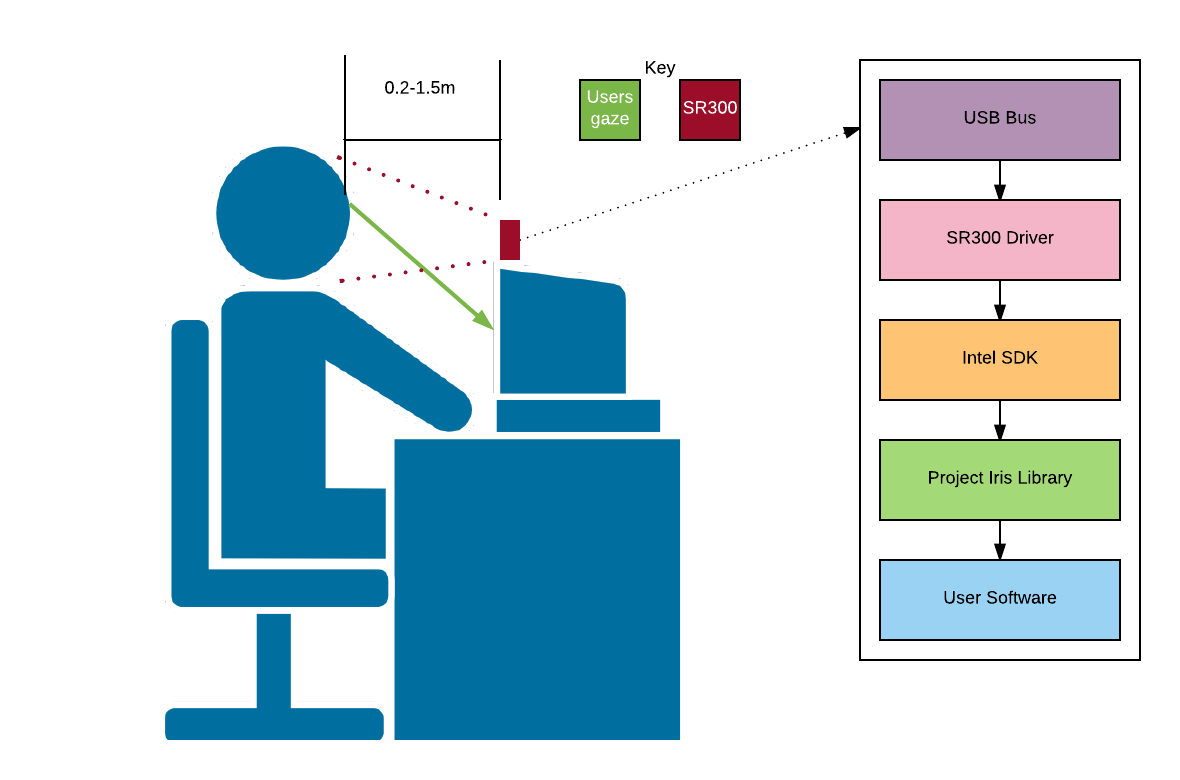
\includegraphics[width=0.60\textwidth]{images/project-iris-system-block}
    \caption{Project Iris system block diagram example}
\end{figure}
